\label{sec:model}

%\begin{figure}
%\centering
%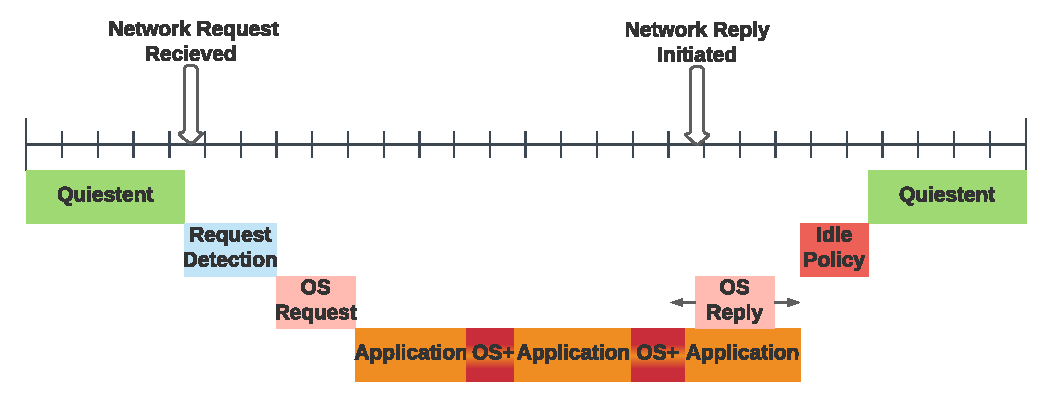
\includegraphics[width=0.5\textwidth]{figures/timeline_chart}
%\caption[]{Logical execution timeline for a single application request}
%\label{fig:timeline}
%\end{figure}

\subsection{Equations}

Using the timeline shown in figure \ref{timeline}, the total time between two consecutive requests arriving at an arrival rate (in queries/requests per unit time) $\lambda$, can be decomposed as:

$\boxed{\delta t = t_{\text{detect}} + t_{\text{osreq}} + t_{\text{app}} + t_{\text{idlepolicy}} + t_q} = \frac{1}{\lambda}$

where 

$\delta t$ = time between the arrivals of two consecutive requests, $t_{\text{detect}}$ = blah, $t_{\text{osref}}$ = blah, $t_{\text{app}}$ = blah, $t_{\text{idlepolicy}}$ = blah, and $t_q$ = blah.

These terms can be grouped together to define:

$t_{\text{work}} \equiv t_{\text{osreq}} + t_{\text{app}} + t_{\text{idlepolicy}}$ for the total time spent on the workload excluding detection and any quiescient time, and $t_{\text{latency}} \equiv t_{\text{detect}} + t_{\text{work}}$ for the total latency for a request.

Note that: $\delta t = \frac{1}{\lambda}$ or equivalently, $t_q = \left[\frac{1}{\lambda} - t_\text{work} - t_{\text{detect}}\right]^+$ where $[x]^+ = \max(x,0)$.


Similarly the total energy consumed during the inter-arrival time, $\delta t$ is:

$\boxed{E = P_\text{detect} t_{\text{detect}} + P_{\text{work}} \left[t_{\text{osreq}} + t_{\text{app}} + t_{\text{idlepolicy}}\right] + P_q t_q} = P_\text{detect} t_{\text{detect}} + P_{\text{work}} t_{\text{work}} + P_q t_q$

Lastly, we posit power-law dependence of $t_{\text{work}}$ and $P_{\text{work}}$ as follows:

$t_{\text{app}} = A\frac{N_i}{\Delta^{1+\alpha}}$

$P_{\text{work}} = B \Delta^{2+\beta}$

where A, B are constants of proportionality, $N_i$ = the total number of instructions and $\alpha$, $\beta$ are real-valued constants that describe the dependence on DVFS, \Delta.

The core assumption here is that the various terms in figure \ref{timeline} don't overlap. We also assume that $\lambda$ is small enough that the latency is less than the inter-arrival time i.e. $t_{\text{latency}} \leq \delta t$. This simple model also applies to the closed-loop case with the restriction that the arrival rate is now dependent on $t_{\text{latency}}$. Lastly, this is a qualitative model that ignores stochastic effects (i.e. the full probability distribution of various terms). A quantitative extension of this analysis would cast this problem as a probabilistic graphical model and perform Bayesian inference for the underlying parameters.

